%!TEX root = ../../Main.tex
\graphicspath{{Chapters/Project/}}
%-------------------------------------------------------------------------------

\chapter{Project}

The project for this reading course is chosen to be carried out using the deep learning framework Caffe. The framework is well known in the deep learning community. It is a rather simple way to obtain a classification convolutional neural network in a very short time, which is the reason why it has been chosen.

The idea of this project is to try out some different neural networks with different values for it's hyperparameters and to see which values will obtain the highest accuracy when training and testing on the CIFAR-10 image data set.

The convolutional network used for inspiration is the one introduced in "Alex's CIFAR-10 tutorial, Caffe style"\footnote{http://caffe.berkeleyvision.org/gathered/examples/cifar10.html} provided by the team behind Caffe. This convolutional network and the changes made to it will be described later on in this chapter along with the architecture and the different types of layers.

%!TEX root = ../../Main.tex
\graphicspath{{Chapters/Project/}}
%-------------------------------------------------------------------------------

\section{Caffe} % (fold)
\label{sec:caffe}

Convolutional Architecture for Fast Feature Embedding (Caffe) is a public available framework which makes it possible to design, train and use a convolutional network in a rather simple way. The source code is available online and the team behind the framework encourage other people to note or change any errors which they might find. The framework allows you to choose to use either the CPU or the GPU for calculations. In this project the CPU is used.

In order to use Caffe for image classification three files are needed - a .prototxt file, a \_solver.prototxt file and a .sh file. These three files together defines the architecture of the network, the hyperparameters and the training and testing strategy.

The .prototxt file defines the architecture of the model e.g. the number and types of layers. An example of a defined layer is shown in \autoref{lst:conv1layer}. The layer exists of three layers - the convolutional layer, the pooling layer and the relu layer. The properties of the different type of layers is described in \autoref{sec:convolutional_network_architecture}.

The three layers are defined with a name, a type, the input (bottom) and the output (top). Some layers has a number of parameters (convolution\_param and pooling\_param) which sets some hyperparameters for the layer.

\begin{lstlisting}[caption = A code snippet from the file  cifar10\_quick\_train\_test.prototxt from the Cifar-10 tutorial provided by the framework. This code snippet defines the first convolutional layer in the network., label={lst:conv1layer}]
layer {
  name: "conv1"
  type: "Convolution"
  bottom: "data"
  top: "conv1"
  param {
    lr_mult: 1
  }
  param {
    lr_mult: 2
  }
  convolution_param {
    num_output: 32
    pad: 3
    kernel_size: 7
    stride: 1
    weight_filler {
      type: "gaussian"
      std: 0.0001
    }
    bias_filler {
      type: "constant"
    }
  }
}
layer {
  name: "pool1"
  type: "Pooling"
  bottom: "conv1"
  top: "pool1"
  pooling_param {
    pool: MAX
    kernel_size: 3
    stride: 2
  }
}
layer {
  name: "relu1"
  type: "ReLU"
  bottom: "pool1"
  top: "pool1"
}
\end{lstlisting}

The \_solver.prototxt file defines how the network is trained. An example of this file is shown in \autoref{lst:solver_prototxt_file}. This file sets the file path for the network to be trained and how often and with how many iterations a test of the network should be carried out.

The file also sets the hyperparameters for the training such as the learning
rate, the momentum, the weight decay and how many iterations and thereby epochs the training should be carried out in. The setting of whether the training should use the GPU or the CPU is also set in this file. From this file it is also possible to set a snapshot file path where the framework can save a snapshot (from a state under the training).

\begin{lstlisting}[caption = The code from the cifar10\_quick\_solver.prototxt from  the Cifar-10 tutorial provided by the framework. This file defines the hyperparameters for the training of the network., label={lst:solver_prototxt_file}]
# reduce the learning rate after 8 epochs (4000 iters) by a factor of 10
# The train/test net protocol buffer definition
net: "examples/cifar10/cifar10_quick_train_test.prototxt"
# test_iter specifies how many forward passes the test should carry out.
# In the case of MNIST, we have test batch size 100 and 100 test iterations,
# covering the full 10,000 testing images.
test_iter: 100
# Carry out testing every 500 training iterations.
test_interval: 500
# The base learning rate, momentum and the weight decay of the network.
base_lr: 0.001
momentum: 0.9
weight_decay: 0.004
# The learning rate policy
lr_policy: "fixed"
# Display every 100 iterations
display: 100
# The maximum number of iterations
max_iter: 4000
# snapshot intermediate results
snapshot: 0
snapshot_prefix: "examples/cifar10/cifar10_quick"
# solver mode: CPU or GPU
solver_mode: CPU
\end{lstlisting}

The .sh file is the executable file which is run to start training. This file contains a few lines which yields which \_solver.prototxt file should be used to train. An example of such a file can be seen in \autoref{lst:train_quick_file}.

\begin{lstlisting}[caption = The code from the train\_quick.sh file from  the Cifar-10 tutorial provided by the framework. This file is executable and yields which \_solver.prototxt file to us to start training., label={lst:train_quick_file}]
#!/usr/bin/env sh

TOOLS=./build/tools

\$TOOLS/caffe train \
  --solver=examples/cifar10/cifar10_quick_solver.prototxt
\end{lstlisting}

The result of the training is a .caffemodel file which contains the parameters of the trained network. This file can be used to classify new images.

% section caffe (end)
%!TEX root = ../../Main.tex
\graphicspath{{Chapters/Project/}}
%-------------------------------------------------------------------------------

\section{CIFAR-10} % (fold)
\label{sec:cifar_10}

The dataset used to train and test the convolutional network on in this project is chosen to be the CIFAR-10 dataset. This dataset is a labeled subset of the much larger tiny image dataset (which contains 80 million tiny images). The collecting has been done by Alex Krizhevsky, Vinod Nair, and Geoffrey Hinton.

The CIFAR-10 dataset consists of 60,000 images spread among 10 classes. The classes are the following: airplane, automobile, bird, car, deer, dog, frog,, horse, ship and truck. The images are of size 32$\times$32 pixels and are colour images.

The dataset is split into a training part and a test part. The training part of the dataset is 50,000 images split into five training batches which contains 10,000 random images each. The test part of the dataset contains exactly 1,000 images from each class which results in a total number of 10,000 images.

The dataset can be downloaded from Alex Krizhevsky's home page\footnote{https://www.cs.toronto.edu/~kriz/cifar.html}.

% section cifar_10 (end)
%!TEX root = ../../Main.tex
\graphicspath{{Chapters/Project/}}
%-------------------------------------------------------------------------------

\section{Convolutional Network architecture} % (fold)
\label{sec:convolutional_network_architecture}

A convolutional neural network exists of a number of different layers with different properties. The different layers used in the networks in this project are described in this section. 

\subsection{Convolutional layers} % (fold)
\label{sub:conv_layers}

The convolutional layers are often the first layers in the network.

Der skal nok skrives lidt om her ..

The Rectified Linear Unit (ReLU) is one of many activation function to choose
among. The ReLU activation function is the most common activation function in the lower layers of convolutional neural netorks. Other activation functions could be the Sigmoid or the Tanh activation functions.

The ReLU differs from the other mentioned activations function in several ways. First of all it converges faster which results in shorter training time. Second of all the ReLU activation function do not saturate which avoids the problem about the gradient getting killed which would lead to the case where the network stops learning during the training (HENVIS TIL MATERIALE OM AKTIVERINGS FUNKTIONER). This problem is known from the use of the other activation functions. 

The formula for the ReLU activation function is $f(x)=max(0,x)$ and is illustrated in FIGURE..

INDSÆT FIGUR

% subsection conv_layers (end)

\subsection{Pooling layers} % (fold)
\label{sub:pool_layers}

Pooling layers are common in-between successive convolutional layers. The primary purpose of introducing pooling layers is to reduce the spatial dimensions of a volume thus alleviating computations needed when training the network. This parameter reduction is achieved by performing a downsampling. Different downsampling strategies exists, e.g. max pooling, average pooling and L2 pooling. 

more fun to come\ldots

overfitting..

% subsection pool_layers (end)

\subsection{Fully-Connected Layers} % (fold)
\label{sub:fc_layers}

% subsection fc_layers (end)

% section convolutional_network_architecture (end)

%!TEX root = ../../Main.tex
\graphicspath{{Chapters/Project/}}
%-------------------------------------------------------------------------------

\section{Training and testing} % (fold)
\label{sec:training_and_testing}

De forskellige hyperparametre, regularization, mini ba, epoches, 

% section training_and_testing (end)
%!TEX root = ../../Main.tex
\graphicspath{{Chapters/Project/}}
%-------------------------------------------------------------------------------

\section{The networks} % (fold)
\label{sec:the_networks}

\subsection{The original network} % (fold)
\label{sub:the_original_network}

Beskrivelse af arkitekturen og implementationsfilerne

Beskrivelse af resultaterne

% subsection the_original_network (end)

\subsection{Another network} % (fold)
\label{sub:another_network}

Beskrivelse af arkitekturen og implementationsfilerne

Beskrivelse af resultaterne

% subsection another_network (end)

% section the_networks (end)
%!TEX root = ../../Main.tex
\graphicspath{{Chapters/Project/}}
%-------------------------------------------------------------------------------

\section{Results} % (fold)
\label{sec:results}

Sammendrag af alle resultater

\vspace{3 mm} % add some space above the table
\begin{table}[H]
\centering
\sffamily
\small
\begin{tabular}{l | c r}
\toprule
Name 					& 4000 iterations		& 8000 iterations	\\
\midrule 
The initial CNN 		& 0.7227				& 0.7191			\\ 
Our AlexNet 			& -- 					& 0.6992	 		\\ 
CNN + add. conv. layer	& 0.7186				& --				\\ 
\bottomrule 
\end{tabular}
\caption[Short caption]{Results}
\label{table:table_results}
\end{table}

% section results (end)
%!TEX root = ../../Main.tex
\graphicspath{{Chapters/Project/}}
%-------------------------------------------------------------------------------

\section{Discussion} % (fold)
\label{sec:discussion}

We have experimented with different configurations in the Caffe framework for
convolutional neural networks as explained in \autoref{sec:networks}. These
experiments resulted in three different networks: The initial CNN, The CNN with
additional convolution layer and The customized AlexNet. Our hypothesis for our
networks were to improve the performance by adding layers and mimicking
a the architecture of a well known CNN. Despite our effort to improve our
networks - based on literature from cs231n \cite{cs231n}, the AlexNet
article\cite{AlexNet} and the article by Zeiler and Fergus \cite{ZeilerFergus} -
the accuracy for the initial CNN on 0.7227 using 4000 iterations is the best result that we could obtain in the experiments.


One of the reasons why our customized AlexNet did not perform as intented could
be our choise of lowering the different parameters in order to be able to use
the AlexNet architecture on the CIFAR-10 dataset. 

% section discussion (end)
%!TEX root = ../../Main.tex
\graphicspath{{Chapters/Project/}}
%-------------------------------------------------------------------------------

\section{Conclusion} % (fold)
\label{sec:conclusion}

We have tried out different convolutional neural network configurations in the
deep learning framework Caffe and we have trained, validated and tested the
configurations on the CIFAR-10 dataset. 


% section conclusion (end)

% \begin{figure}[H]
% \centering
% 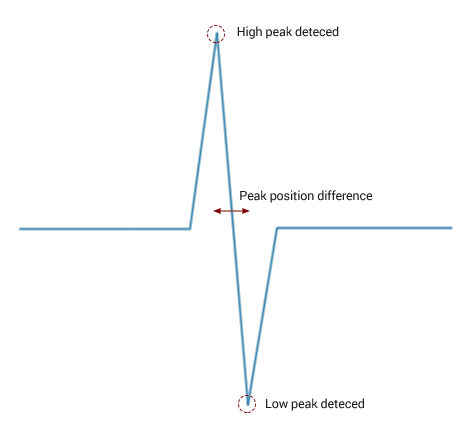
\includegraphics[width = 200 pt]{Img/Figures.png}
% \caption{Block diagram}
% \label{fig:BlockDiagram}
% \end{figure}
% 
% \begin{equation}
% \frac{n!}{k!(n-k)!} = \binom{n}{k}
% \label{eq: myequation}
% \end{equation}